\begin{problem}{트리 회전}
	{standard input}{standard output}
	{1 second}{128 megabytes}{}
	
	
	정원사 범수는 `한탄의 나무'라는 이름의 희귀한 나무를 기르고 있다. 이 나무는 몇몇 특징들이 있다.
	
\begin{itemize}
\item 나무는 곧은 가지와 잎으로 이루어져 있다. 땅에서 나온 줄기도 가지라고 말한다.
\item 각 가지는 분기점이나 잎으로 끝난다. 
\item 가지 끝에 있는 분기점은 왼쪽 가지와 오른쪽 가지의 두개의 가지로 나뉘어 진다.
\item 나무에 있는 모든 잎은 1부터 $n$까지의 번호가 붙어있다. 모든 잎에 붙은 번호는 유일하다.
\item 범수는 `회전'을 통해 분기점에 있는 왼쪽 가지와 오른쪽 가지를 바꿀 수 있다.
\end{itemize}

한탄의 나무의 `한탄수열'은 왼쪽에서 오른쪽으로 잎에 쓰인 정수들을 읽어 만들어진 수열이다.

범수는 지구이웨에 오래 살았고, 다른 지구이웨에 사는 사람처럼 깔끔함과 질서를 사랑한다. 그는 자기가 기르는 나무가 `회전'을 통해 얼마나 깔끔해 질 수 있는지가 궁금해 졌다. 나무의 깔끔함은 한탄수열의 반전계수로 정해진다. 어떤 수열 $a_1,a_2,\cdots,a_n$의 반전 계수란 $1 \le i < j \le n$ 이면서 $a_i > a_j$ 인 ($i$, $j$) 쌍의 갯수이다.

\vspace{5mm}
\begin{center}
	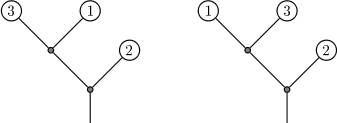
\includegraphics[]{rot.png}
\end{center}
\vspace{5mm}
	
	왼쪽에 있는 원래 나무는 한탄수열이 3, 1, 2였고 반전계수가 2였다. 회전을 한 번 하면 오른쪽 나무로 바뀐다. 이 나무의 한탄수열은 1, 3, 2가 되었고, 반전 계수는 1이 되었다. 각 나무는 5개의 가지가 있다.
	
	범수가 트리를 적당히 회전해서 만들 수 있는 한탄수열의 반전계수의 최솟값을 찾아라.

	\InputFile
	
	입력에 첫째 줄에는 범수의 나무에 있는 잎의 갯수 $n$이 주어진다. ($2 \le n \le 200,000$)
	
	그리고, 다음은 재귀적으로 정의된 나무가 주어진다.
	
	\begin{itemize}
		\item $p$ 로 끝나는 잎이 가지 끝에 있다면, 하나의 정수 $p$가 입력으로 주어진다. ($1 \le p \le n$)
		\item 가지 끝이 분기점이라면, 트리는 다음과 같이 주어진다.
		\begin{itemize}
			\item 첫째 줄에는 0이 주어진다.
			\item 그리고 왼쪽 가지에 달린 나무가 주어진다. (분기점을 땅이라고 생각하고 주어진다.)			\item 그리고 오른쪽 가지에 달린 나무가 주어진다. (분기점을 땅이라고 생각하고 주어진다.)
		\end{itemize}
	\end{itemize}
	

	
	\OutputFile
	
	첫째 줄에 범수가 트리를 적당히 회전해서 만들 수 있는 한탄수열의 반전계수의 최솟값을 출력한다.
	
	\SubtaskWithCost{1}{30}
	\begin{itemize}
		\item $n \le 5,000$
	\end{itemize}
	
	\SubtaskWithCost{2}{70}
	
	추가 제한 조건이 없다.
	
	\Examples
		
	\begin{example}
	\exmp{
		3
		0
		0
		3
		1
		2
		
	}{%
	1
	}%
	\end{example}

	\Note
	
	그림의 왼쪽에 있는 나무는 예제에서 주어진 나무이다.
	
\end{problem}

